% !TeX spellcheck = en_GB

\documentclass[preprint,12pt]{elsarticle}
\usepackage{graphicx,psfrag,epsf}
\usepackage{amsfonts}
\usepackage{mathtools}
\usepackage{amssymb}
\usepackage{amsmath}
\usepackage{longtable}
\usepackage{bigints}
\usepackage{soul}
\usepackage{tikz}
\usetikzlibrary{arrows.meta}
\tikzset{>={Stealth[length=3mm]}} % better arrow heads
\usepackage{color}

\usepackage{hyperref}
\usepackage[capitalise]{cleveref}
\usepackage{url}
\usepackage{doi}
\usepackage{multicol}
\usepackage{multirow}
\usepackage{subcaption}

\newcommand{\x}{\boldsymbol{X}}
\renewcommand{\b}{\hat{\beta}}
\newcommand{\reals}{\mathbb{R}}
\newcommand{\normal}{\mathcal{N}}
\newcommand{\lexp}{\underline{\mathbb{E}}}
\newcommand{\uexp}{\overline{\mathbb{E}}}

\usepackage{lineno}
\linenumbers

\begin{document}

\begin{frontmatter}

%%% MT to TB: what about "Robust Bayesian Analysis of Causal Inference in Medical Diagnosis and Treatment"
%%% TB to MT: changed it
\title{Robust Bayesian Analysis of Causal Inference in Medical Diagnosis and Treatment}
\author[1]{Tathagata Basu\corref{cor1}}
\ead{tathagatabasumaths@gmail.com}
\cortext[cor1]{Corresponding author}
\author[2]{Matthias C.~M.~Troffaes}
\ead{matthias.troffaes@durham.ac.uk}
\affiliation[1]{organization={Civil and Environmental Engineering, University of Strathclyde},
            addressline={16 Richmond St}, 
            city={Glasgow},
            postcode={G1 1XQ}, 
            %state={},
            country={United Kingdom}}
\affiliation[2]{organization={Department of Mathematical Sciences, Durham University},
            addressline={South Road}, 
            city={Durham},
            postcode={DH13LE}, 
            %state={},
            country={United Kingdom}}

\begin{abstract}
Causal inference aims to find the causal effect on subjects
by identifying causal links between
a number of predictor (or, explanatory) variables and the outcome of a treatment.
However, estimation of such causal links is extremely 
difficult because the causal effects may vary from subject 
to subject. Unfortunately, modelling the underlying heterogeneity explicitly makes the 
problem practically unsolvable. Additionally, for high dimensional problems,
we often need to find a subset of 
predictor variables to initiate the treatment. However, current variable selection methods
simply tend to maximise the predictive performance of the outcome model. This can be problematic when information and data are limited,
as the consequence of mistreatment can be harmful. 
So, in this paper, we develop a model for causal inference using
robust Bayesian analysis, to allow for abstention when selecting
predictor variables.
We
use a set of spike and slab priors 
through prior elicitation to obtain robust estimates for
both the treatment and outcome model. We are specifically interested 
in the sensitivity of the causal effect in high dimensional causal inference
as well as identifying predictor variables that are causally linked. However, indicator
based variable selection can be deceptive, especially
when the predictor is strongly associated with either the treatment or 
the outcome, as this increases the posterior expectation of the selection
indicators. To avoid that, we apply a post-hoc selection scheme
which successfully removes negligible non-zero effects from the model,
attaining a smaller set of 
predictors.
Finally, we illustrate
our method using a synthetic dataset.
\end{abstract}

\begin{keyword}
  high dimensional data\sep variable selection\sep Bayesian analysis\sep imprecise probability
\end{keyword}

\begin{highlights}
\item *** TODO ***
\item *** TODO ***
\end{highlights}

\end{frontmatter}

\section{Introduction}\label{sec:intro}

Causal inference using observational data is important in
many fields, including epidemiology, social science, economics, and many more.
Causal inference concerns estimating the causal
effect of predictor variables on an outcome variable,
as well as identifying which predictors are causally linked with the outcome.
Ideally,
randomised trials are the most efficient way to perform this task.
However, this is not always practical due to, for instance, ethical 
concerns, design cost, population size, to name a few. This
leaves us with observational studies
where data is collected though surveys or record keeping.

But this
can be problematic in the presence of confounding.
\begin{figure}
\begin{center}
\begin{tikzpicture}[node distance=2cm, auto]
  \node (confounder) at (0,0) [circle,draw,align=center] {biomarker \\(confounder)};
  \node (predictor) at (4,2) [circle,draw,align=center] {treatment \\ decision \\ (predictor)};
  \node (outcome) at (4,-2) [circle,draw,align=center] {treatment \\ outcome};
  \draw[->] (confounder) to (predictor);
  \draw[->] (confounder) to (outcome);
  \draw[->,dashed] (predictor) to (outcome);
\end{tikzpicture}
\end{center}
\caption{A biomarker influencing both the treatment decision and the treatment outcome, thereby acting as confounder. Solid arrows indicate causation, whilst the dashed arrow indicates correlation without causation.}
\label{fig:confounding}
\end{figure}
A confounder is any variable which is causally linked with both a predictor and the outcome, giving the false impression that that predictor causes the outcome (see \cref{fig:confounding}).
Confounding happens commonly in observational treatment studies because many predictors are often causally linked with the treatment decision (which is also a predictor), whilst simultaneously affecting the outcome of the treatment. Any such predictors act as a confounders between treatment decision (as one of the predictor variables) and treatment outcome.
In such cases, we must be extra cautious as we risk
unwanted bias in the causal effect estimator \citep{rosenbaum83},
if we ignore such correlations.
Several authors have tackled the presence of
confounder variables. 
\Citet{Robins1986ANA} used a graphical
approach to identify the causal parameters.
\Citet{rosenbaum1985} suggested a link model to estimate
the propensity scores for all individuals. Subsequently, several other
methods have been proposed based on propensity score matching;
see \citep{winship99,stuart10} for a brief review.

One of the earlier Bayesian approaches to causal inference
can be found in \citep{rubin1978}. More recently,
with the rise of high dimensional data,
Bayesian methodologies have grown in popularity.
\Citet{Crainiceanu2008} proposed a bi-level 
Bayesian model averaging based method for estimating the causal 
effect. \Citet{wang2015} suggested BAC (or, Bayesian adjustment for
confounding),
where an informative prior obtained from
the treatment model is applied on the outcome model for
estimating the causal effect. Several other methods were
proposed to tackle confounders from a Bayesian perspective,
see for instance \citep{Zigler2014,Hahn2018} among others.

In this paper we take inspiration from the approach of \citet{koch2020}, who proposed a bi-level spike and slab prior for causal effect 
estimation. They considered a data-driven adaptive approach to
propose their prior which reduces the variance of the causal estimate. 
Our approach is based on
sensitivity analysis, where instead of using a single prior, 
we consider a set of priors \citep{BERGER1990303}. %TB to MT: added zaffalon paper
Some works have been done in this approach of
prior sensitivity analysis. \citet{zaffalon20a} 
used credal networks in structured causal models
for causal inference; \citet{raices_cruz22} suggested
that causal effect estimation can be performed 
through a meta analysis where robust Bayesian analysis 
can be beneficial under severe uncertainty. 
This motivates us to extend prior sensitivity analysis for 
regression models. This is particularly beneficial, as for high dimensional regression problems 
we have to rely on very limited data to perform our Bayesian analysis and 
inference with a single prior
is unreliable.
To perform a prior sensitivity analysis, we use expert opinion to elicit a set of priors 
based on empirical evidence. 
This allows us to construct the problem of 
predictor selection
in a framework where abstention has a relatively positive gain i.e.~
when the cost of further tests/data collection is cheaper than
mistreating a subject.

Our framework considers a set of continuous spike and slab priors 
\citep{ishwaran2005} for
predictor selection.
We thereby construct a Bayesian group LASSO \citep{xu2015} type problem.
To perform sensitivity analysis,
we consider a set of beta priors on the covariate selection 
probability of the spike and slab priors. We use the posteriors of this
covariate selection probability for identifying the active predictors. Finally, 
we consider a post-hoc coefficient adjustment method \citep{hahn2015}
to recover sparse estimates associated with either the outcome or the
treatment model. 

The rest of the paper is organised as follows. In \cref{sec:causal}
we give a formal description of the causal estimation problem in the
context of linear regression. \Cref{sec:bayes} is focused on the
Bayesian analysis of causal inference problems, followed by the
motivation of a robust Bayesian analysis along with our proposed decision 
theoretic framework for predictor selection. In \cref{sec:sim}, 
we provide results of simulation studies under different scenarios 
and show the possible applications in real life problems. Finally, 
we discuss our findings and conclude this paper in \cref{sec:conc}.

\section{Causal Estimation}\label{sec:causal}

\subsection{Regression Model}

Let an observational study on $n$ individuals give us
\emph{treatment outcomes} $Y\coloneqq(Y_1, \dots, Y_n)$ with 
corresponding \emph{treatment decisions} $T\coloneqq(T_1, \dots, T_n)$.
Here, we use an indicator to represent the treatment decision. That is, $T_i$ is $1$ if the $i$th patient was treated, and $0$ otherwise. Similarly,
$Y_i$ is the treatment outcome of the $i$th patient, represented as some real-valued quantity.

Regression methods are widely used in causal effect estimation. The
main idea behind these regression methods is to remove the
correlation between the treatment indicator and the error term
\citep{winship99,HECKMAN1985}.
To do so, we rely on $p$ observed quantities, called
\emph{predictors}, denoted by $X\coloneqq$ $[X_1^T, \dots, X_n^T]^T$
where each $X_i\in\mathbb{R}^p$.
Each $X_i$ is treated as a $p$-dimensional row vector,
so $X$ is a $n\times p$ matrix.
Now, let
$\beta \coloneqq (\beta_1$, \dots, $\beta_p)^T$ denote the vector of regression
coefficients
related to the predictors, and let $\beta_T$ denote a regression coefficient related to the
treatment decision.
Then we can define a linear model for the outcome
so that
\begin{equation}
	Y_i =  T_i \beta_{T} + X_i\beta + \epsilon_i
\end{equation}
where $\epsilon_i\sim \mathcal{N}(0, \sigma^2)$,
independent of $T_i$ and $X_i$.
Note that both $T_i$ and $X_i$ are predictors for $Y_i$ in the above model.
However, when we talk about predictors in this paper, we usually mean just the components of $X_i$.

To decide whether or not to treat a new individual with given predictors,
we are mainly interested in the effect of the treatment on the outcome.
More precisely, the causal effect of a new individual, indexed as $n+1$,
whose outcome $Y_{n+1}$ is not yet observed, and with observed predictors $X_{n+1}=x_{n+1}$, is defined by:
\begin{align}
  \delta(x_{n+1})
  &\coloneqq\mathbb{E}(Y_{n+1}\mid X_{n+1}=x_{n+1},T_{n+1} =1) - \mathbb{E}(Y_{n+1}\mid X_{n+1}=x_{n+1},T_{n+1}=0)
\end{align}
For our model, due to linearity of expectation, we have that
\begin{align}
  \delta(x_{n+1})
  &=\beta_T+x_{n+1}\beta+\mathbb{E}(\epsilon_{n+1}\mid X_{n+1}=x_{n+1},T_{n+1} =1) \\
  &\quad - x_{n+1}\beta-\mathbb{E}(\epsilon_{n+1}\mid X_{n+1}=x_{n+1},T_{n+1} =0)\\
  \intertext{and because $\epsilon_{n+1}$ is independent from $X_{n+1}$ and $T_{n+1}$,}
  &=\beta_{T}.
\end{align}
Note that, for this model, the causal effect $\delta(x_{n+1})$
does not depend on the observed value $x_{n+1}$ of $X_{n+1}$.
So, to find the causal effect, we simply need to estimate $\beta_T$.

To estimate $\beta_T$ from the data $X$, $Y$ and $T$,
especially in the presence of confounders,
we also need to consider the
association between the treatment indicators $T$ and the predictors $X$.
A common choice in the literature is to use a probit link function.
In this way, we can
specify the conditional probability that subject $i$ receives the treatment through a linear model. 
That is, for another vector of regression coefficients 
$\gamma\coloneqq(\gamma_1, \cdots, \gamma_p)^T$ we
assume
\begin{align}
	P(T_i=1\mid X_i) = \Phi(X_i\gamma)
\end{align}
where $\Phi$ denotes the cumulative distribution function
of a standard normal distribution. To incorporate this probit
link function, we model the $T_i$ as follows \citep{albert93}:
\begin{align}
    T_i^* &= X_i\gamma +u_i \\
    T_i   &= \mathbb{I}(T_i^*>0)
    =
    \begin{cases}
    1 & \text{if }T_i^*>0 \\
    0 & \text{otherwise}
    \end{cases}
\end{align}
where $u_i\sim\mathcal{N}(0,1)$.
With this model, indeed
\begin{align}
  P(T_i=1\mid X_i)
  &=P(T_i^*>0)=P(u_i>-X_i\gamma)=1-P(u_i\le -X_i\gamma) \\
  &=1-\Phi(-X_i\gamma)=\Phi(X_i\gamma)
\end{align}

Now, to construct the joint likelihood function, we define an extended
output $2n\times 1$ column vector
$W\coloneqq\left(\begin{smallmatrix}Y \\ T^*\end{smallmatrix}\right)$
and corresponding $2n\times(2p+1)$ dimensional design matrix
\begin{align}
	Z &\coloneqq
        \begin{bmatrix}
           T_1 & X_1 & 0 \\
           \vdots & \vdots & 0 \\
           T_n & X_n & 0 \\
           0 & 0 & X_1 \\
           \vdots & \vdots & \vdots \\
           0 & 0 & X_n
        \end{bmatrix}
        =
	\begin{bmatrix}
		X_O & 0 \\
		0 & X_T
	\end{bmatrix}
\end{align}
where, $X_O \coloneqq [T, X]$ and $X_T \coloneqq X$. Then, considering the assumption of
Gaussian error terms, we have the following likelihood distribution
\begin{align}
	W\mid Z, \beta_T, \beta, \gamma, \sigma^2 \sim\normal\left(Z\nu, \Sigma\right)\label{eq:like:group},
\end{align}
where $\nu \coloneqq (\beta_T, \beta^T, \gamma^T)^T$ and
\begin{align}
	\Sigma &\coloneqq
	\begin{bmatrix}
		\sigma^2{I}_n & 0 \\
		0 & {I}_n
	\end{bmatrix}.
\end{align}


\section{Bayesian Causal Estimation}\label{sec:bayes}

The likelihood given by \cref{eq:like:group} gives us
a foundation for a Bayesian group LASSO 
\citep{xu2015} type model. In this way, we can look into the posterior selection
probability of each predictor. There are several
ways to construct spike and slab priors for
variable selection. Here, we consider a continuous type
prior \citep{ishwaran2005} for faster posterior
computation.


\subsection{Hierarchical model}

Let $\pi_j$ denote the prior probability that the $j$-th
predictor is associated with the outcome or the 
treatment. That is, conceptually,
\begin{equation}
	\pi_j \coloneqq P\left((\beta_j,\gamma_j)\not=(0,0)\right).
\end{equation}
Practically, we model this by defining the following hierarchical model
so that,
for $1\le j\le p$,
\begin{align}
	\label{eq:spike:slab:prior:beta:gamma}(\beta_j,\gamma_j)^T \mid \pi_{j}, \sigma^2 &\sim 
	\pi_{j}\normal\left( \begin{bmatrix}
		0 \\
		0
	\end{bmatrix}, 
	\tau_1^2\begin{bmatrix}
		\sigma^2 & 0 \\
		0 & 1
	\end{bmatrix}\right)
	+ (1-\pi_{j}) \normal\left(\begin{bmatrix}
		0 \\
		0
	\end{bmatrix}, 
	\tau_0^2\begin{bmatrix}
		\sigma^2 & 0 \\
		0 & 1
	\end{bmatrix}\right)\\
	\beta_T\mid \sigma^2 &\sim \normal\left(0, \sigma^2\right)\\
        \frac{1}{\sigma^2}&\sim \text{Gamma}(a, b)\\
	\pi_{j} &\sim\text{Beta}\left(sq_j, s(1-q_j)\right).
\end{align}
In the hierarchical model, we fix sufficiently small $\tau_0$
$(1\gg\tau_0>0)$ so that  $(\beta_j, \gamma_j)$ has its probability mass 
concentrated around zero. Therefore, this represents the spike component of our prior specification. 
For the slab component, we consider $\tau_1$ to be large so that $\tau_1\ge 1$. This allows the prior for $(\beta_j,\gamma_j)$ to be flat beyond the spike component at the origin. 
We illustrate the components of a bivariate spike and slab prior in 
\cref{fig:ssbl} (with fixed $\sigma=1$). We generate the spike component 
with $\tau_0=0.001$ and the slab component with $\tau_1=5$.

\begin{figure}[h]
	\begin{center}
		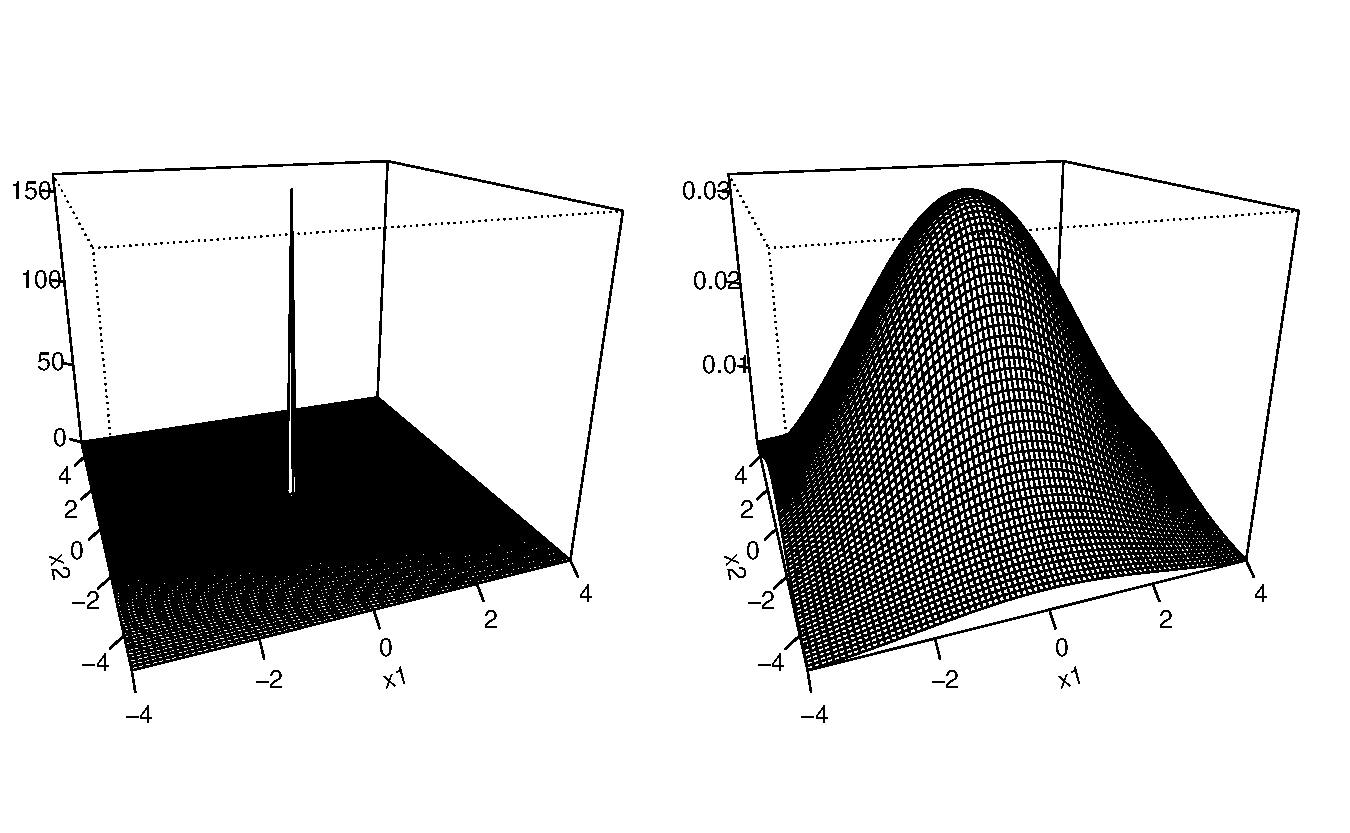
\includegraphics[width = 0.95\linewidth]{spike_slab_bi.pdf}
	\end{center}
	\caption{Spike (left) and slab (right) components of a bivariate distribution for $\tau_0 = 0.001$, $\tau_1$ = 5 and $\sigma=1$.}
	\label{fig:ssbl}
\end{figure}

For the precision term $1/\sigma^2$, a natural choice of prior is the gamma distribution
as it allows the control of both the location and the scale of the precision.
To ensure that the prior is able to represent the data, we consider $b=1$ and 
fix $a$ so that it represents the prior mean of the precision.
Alternatively, when $b=1$, we know that the interval
$[0, 3a]$ contains the true value of the precision parameter with probability close to $0.95$.
So, we can also use a prior judgement on the 95\% quantile to set $a$.
We use a beta prior to
model our uncertainty about
the selection probabilities $\pi_j$ where  $q_j$ represents our prior expectation of $\pi_j$ and $s$ acts as 
a concentration parameter.
For the causal effect, we want to use a Gaussian distribution that 
matches the scale of the noise term. Therefore, we consider $\beta_T\sim \normal(0,\sigma^2)$. 

In \cref{fig:regress}, we show a probabilistic graphical representation
of our hierarchical model. In the figure, grey circular nodes represent the
prior hyper-parameters which will be used for sensitivity analysis
of the model. The transparent circular nodes are used to denote
the modelling parameters which are our quantities of interest. 
The observed quantities are denoted with transparent rectangular
nodes. We also use a grey rectangular node to denote the intermediate
latent variable $T^*$. We use directed edges to denote the
relationship between different nodes. However, we use a dashed
edge between $X$ and $T$ as they are related through the latent
variable $T^*$. 

\begin{figure}
	\centering
	\begin{tikzpicture}[params/.style={circle, draw=black!60, very thick, minimum size=7mm},
		hyper/.style={circle, draw=black!60, fill=black!20, thick, minimum size=7mm},
		post/.style={circle, draw=black!60, fill=green!20, thick, minimum size=7mm},
		latent/.style={rectangle, draw=black!60, fill=black!10, dashed, minimum size=7mm},
		data/.style={rectangle, draw=black!60, thick, minimum size=8mm}]
		\node[params] (1) at (0,0) {$\pi$};
		\node[data] (2) at (3,0) {$X$};
		\node[data] (3) at (6,0) {$T$};
		\node[params] (4) at (1.5,1.5) {$\gamma$};
		\node[latent] (5) at (4.5,1.5) {$T^*$};
		\node[params] (6) at (1.5,-1.5) {$\beta$};
		\node[data] (7) at (3.5,-1.5) {$Y$};
		\node[params] (8) at (0,-3) {$\sigma^2$};
		\node[params] (10) at (6,-1.5) {$\beta_T$};
		\node[hyper] (11) at (-1.5,-.8) {$s$};
		\node[hyper] (12) at (-1.5,.8) {$q$};
		\node[hyper] (13) at (-1.5,-2.2) {$a$};
		\node[hyper] (14) at (-1.5,-3.8) {$b$};
		\draw[black, dashed] (0.75,-3.7) rectangle (7,2.1);
		
		\path (1) edge[->]  (6);
		\path (1) edge[->]  (4);
		\path (8) edge[->]  (6);
		\path (6) edge[->]  (7);
		\path (2) edge[->]  (7);
		\path (2) edge[->]  (5);
		\path (5) edge[<-] (4);
		\path (5) edge[->] (3);
		\path (3) edge[->]  (7);
		\path (10) edge[->]  (7);
		\path (2) edge[dashed][->] (3);
		\path (8) edge[bend right = 60][->]  (10);
		\path (11) edge[->]  (1);
		\path (12) edge[->]  (1);
		\path (13) edge[->]  (8);
		\path (14) edge[->]  (8);
		
	\end{tikzpicture}
	\caption{Probabilistic graphical representation for causal inference with Bayesian hierarchical model.}
	\label{fig:regress}
\end{figure}

\subsection{Robust Bayesian Analysis}

The hierarchical model presented above is a standard spike and slab model for
variable selection and performs well when we have sufficient data. 
However, especially in the case of causal inference, we do not always have sufficient data. Moreover, 
we also must be cautious about the side effects of a treatment.
Therefore, we are particularly interested in constructing a robust Bayesian framework
for variable selection. In this way, when we are preparing guidelines for treatment, we 
can have the option to ask for more data before reaching any conclusion. To achieve this,
we consider a utility based framework with three possible 
scenarios.

In particular, through predictor selection, we also want 
to check if a certain bio-marker should be considered
for the treatment decision. For example, say we can observe blood pressure with some
other bio-markers and want to decide whether our
treatment guideline should also consider the blood
pressure of the subject before treating them. This is
useful as an unnecessary treatment of a subject can have severe consequences because of the medicinal
side effects. In general, it is hard to associate such consequences 
with a suitable loss function. Instead, we
assume that we can always revert any initial mistreatment by further treatments, 
and we can associate a loss function with the cost of further treatments.
So, we will associate two constant loss values $\ell_1$ and $\ell_2$ 
with false positives (falsely selected predictor) and 
false negatives (falsely rejected predictor) respectively. 
Clearly, false positives may lead to unwanted side effects and
false negatives may lead to mistreatment of the patient. Finally, we associate
a loss value $\ell_3$ for abstention from selecting
a variable which can be interpreted as the cost of further tests to determine whether that bio-marker
is important for constructing the treatment guideline.
Ideally, in most cases, $\ell_3\ll \ell_1,\ell_2$. However, in certain scenarios,
this might not be the case, especially when the condition of a subject deteriorates rapidly
over time.

Now, based on this notion of abstaining from selecting a predictor, we can perform
a sensitivity analysis over a set of priors on the prior selection probability.
That is, we can consider a set of possible values for $q$ such that
$q\in\mathcal{P}$, where $\mathcal{P} \subseteq \left(0, 1\right)^{p}$.
Here, the equality occurs for the near vacuous case. However, in real-life
situations, performing a robust Bayesian analysis for the near vacuous case is 
not practical. Instead, we incorporate expert elicitation to define our model.
For instance, we can consider $q\in \left[\underline{q}, \overline{q}\right]$
where $p\underline{q}$ and $p\overline{q}$ represent the bounds of the prior expectation on the
total number of variables present in either of the models.

\subsection{Variable selection and coefficient adjustment}
For the co-variate selection, we look into the posterior expectation of $\pi_j$. 
We consider the $j$-th predictor to be removed from both the
treatment and outcome model, if
\begin{align}\label{eq:vs:remove}
	\uexp (\pi_j\mid W)\coloneqq \sup_{q\in \mathcal{P}} \mathbb{E}_q(\pi_j\mid W) < 1/2.
\end{align}
Similarly, we consider the $j$-th predictor to be present in at least one of the models, if
\begin{align}\label{eq:vs:sel}
	\lexp (\pi_j\mid W)\coloneqq \inf_{q\in \mathcal{P}} \mathbb{E}_q(\pi_j\mid W) \ge 1/2.
\end{align}
Otherwise, we consider the variable to be indeterminate,  in which case we abstain from putting
it in any of the models but instead just report a lack of information.

In general, this framework is
sufficient
for variable selection. However, for
model fitting and prediction, we need to evaluate the values 
of the regression coefficients. For that we first need to find the set of active
predictors with respect to our prior expectation of the selection probability $q$.
For any fixed $q$, we define the set $S(q)$ as the set of all variables which are active
in the treatment model or in the outcome model:
\begin{equation}
	S(q)\coloneqq
	\left\{j\colon \mathbb{E}_q(\pi_j\mid W) \ge 1/2\right\}.
\end{equation}
For sensitivity analysis,
the intersection of $S(q)$ over all $q$ gives us the set of
active variables obtained through \cref{eq:vs:sel}.
Similarly, the union gives us the set of
variables that are not removed through \cref{eq:vs:remove}.
That is:
\begin{align}
    \mathcal{S}_*&\coloneqq \left\{j:\lexp (\pi_j\mid W)\ge1/2\right\}
    = \bigcap_{q\in \mathcal{P}}S(q), \\
    \mathcal{S}^*&\coloneqq \left\{j:\uexp (\pi_j\mid W)\ge1/2\right\}
    = \bigcup_{q\in \mathcal{P}}S(q).
\end{align}
Clearly, $\mathcal{S}_*\subseteq\mathcal{S}^*$.
$\mathcal{S}_*$ represents the set of variables that are sure to be selected,
$\{1,\dots,p\}\setminus\mathcal{S}^*$ represents the set of variables that are sure to be removed, and
$\mathcal{S}^*\setminus\mathcal{S}_*$ represents the set of variables about which we are undecided.
In this way, through sensitivity analysis, our approach incorporates robustness.

We can derive bounds on the posterior means of the parameters as follows:
\begin{align}
\label{eq:beta:lower}
\underline{\beta}_j&\coloneqq\lexp (\beta_j\mid W)= \inf_{q\in \mathcal{P}} \mathbb{E}_q(\beta_j\mid W) \\
\label{eq:beta:upper}
\overline{\beta}_j&\coloneqq\uexp (\beta_j\mid W)=\sup_{q\in \mathcal{P}} \mathbb{E}_q(\beta_j\mid W)
\end{align}
with similar expressions for 
$\underline{\beta}_T$, $\overline{\beta}_T$,
$\underline{\gamma}_j$ and $\overline{\gamma}_j$.
If we take the posterior expectation interval $[0,0]=\{0\}$ on a regression coefficient to represent absence of a variable, then our bounds on the regression coefficients are generally not sparse, because we use continuous 
spike and slab priors.

Moreover, with our variable selection we only determine whether the variable 
is included in at least one of the models.
To determine which predictors
influence the outcome ($\beta_j\neq 0$),
the treatment ($\gamma_j\neq 0$), or both,
and to understand the degree of assocation
(i.e.\ the magnitude of $\beta_j$ and/or $\gamma_j$),
we apply the 
``decoupled shrinkage and selection'' (DSS) method proposed by \citep{hahn2015}. 
For that, we solve the following adaptive LASSO-type \citep{Zou2006}
problems:
\begin{align}
	\hat{\beta}^D_{S(q)} &= 
	\arg\min_{\beta_{S(q)}} \frac{1}{n}\|X_{S(q)}\hat{\beta}_{S(q)}
	- X_{S(q)} \beta_{S(q)}\|_2^2 + \lambda\sum_{j\in S(q)} 
	\frac{|\beta_{j,S(q)}|}{|\hat{\beta}_{j,S(q)}|}
\end{align}
and
\begin{align}
	\hat{\gamma}^D_{S(q)} &= 
	\arg\min_{\gamma_{S(q)}} \frac{1}{n}\|X_{S(q)}\hat{\gamma}_{S(q)}
	- X_{S(q)} \gamma_{S(q)}\|_2^2 + \lambda\sum_{j\in S(q)} 
	\frac{|\gamma_{j,S(q)}|}{|\hat{\gamma}_{j,S(q)}|}
\end{align}
where $q\in \mathcal{P}$,
where $\hat{\beta}_{S(q)}$ 
and $\hat{\gamma}_{S(q)}$ are the posterior means 
of the regression coefficients with respect to
the predictors that belong to $S(q)$.
By varying $q$, this gives us a set of point estimates for the model parameters $\beta$ and $\gamma$, along with a more detailed selection of individual $\beta_j$ and $\gamma_j$.

To compute the posterior bounds (as in \cref{eq:vs:remove,eq:vs:sel,eq:beta:lower,eq:beta:upper}), unfortunately, we usually have to resort to brute force optimisation, due to the lack of tractable expressions for the posterior expectations. 
This is obviously a major drawback of this approach.

\iffalse
The DSS method explained
above give us adjusted coefficient estimates for the treatment
and outcome model. However, as result the causal effect estimate
remains the same and modelling with such adjusted sparse effect 
will contribute to the prediction error. Therefore, we need to 
adjust the causal effect estimate as well. Let
\begin{equation}
    \hat{T}^D = \mathbb{I}\left(X_{S(q)}\hat{\gamma}^D_{S(q)} >0\right)
    \quad\text{and}\quad
    \hat{T} = \mathbb{I}\left(X\hat{\gamma}^q >0\right).
\end{equation}
and let $\beta_{T}^D(q)$
be the causal effect after applying `DSS' and $\hat{\beta}_{T}(q)$ be the
posterior estimate of the causal effect for any fixed $q\in\mathcal{P}$. Then
the adjusted estimate is given by:
\begin{equation}
    \beta_{T}^D(q) = \left(\left(\hat{T}^D\right)^T \hat{T}^D\right)^{-1}
    \left(\hat{T}^D\right)^T \left[\hat{\beta}_{T}(q)\hat{T} 
    + X_{S(q)}\left(\hat{\beta}_{S(q)} - \hat{\beta}^D_{S(q)}\right) 
    +X_{S^C(q)}\hat{\beta}_{S^C(q)}\right]
\end{equation}
where
\begin{equation}
    S^C(q)\coloneqq \left\{1,2,\cdots, p\right\} \neg S(q).
\end{equation}
\fi

\subsection{Refit}

In our setting, the DSS method only gives us a set of point estimates for the final selection of variables: some coefficients may be always selected, some never, and some will be indeterminate. For the final inference model, the modeller will need to make a judgement about which of the indeterminate coefficients $\beta_j$ and $\gamma_j$ to include in the final model or not. Once done so, the model can be refitted to account for the effect of variable selection on the estimation of the model parameters.

To do so, we can again use our Bayesian model without $\pi_j$ (as there is no selection anymore), and with priors
\begin{align}
\beta_j\mid\sigma^2&\sim\mathcal{N}(0,\tau_1^2\sigma^2) \\
\gamma_j\mid\sigma^2&\sim\mathcal{N}(0,\tau_1^2)
\end{align}
for those $\beta_j$ and $\gamma_j$ that are selected in the model, with the remaining $\beta_j$ and $\gamma_j$ set to zero.
This is similar to the spike and slab prior from \cref{eq:spike:slab:prior:beta:gamma} but without the spike component.

We expect this to have only a small effect on the mean and variance of the estimated parameters. This refit is useful to validate the variable selection and to improve the estimating of the model parameters, including the causal effect $\beta_T$. Indeed, since there are fewer parameters for the same data, the estimates are expected to have less uncertainty.

Note that here, we described a precise Bayesian refit model, but obviously this could be extended to robust Bayesian refit models too.

\section{Simulation Studies}\label{sec:sim}

For the simulation studies, we consider 4 different settings. In each
case, we generate the design matrix $X$ such that $X_i\sim\mathcal{N}(0, \Sigma)$
for $1\le i\le n$ where $\Sigma_{ij} = 0.3^{|i-j|}$. In this way, we 
generate predictors for our model with mild correlations between them.
We then use the following distributions to generate the outcome and
the treatment indicator: 
\begin{equation}
    T_i \sim \text{Bernoulli}\left(1/(1+\exp(-X_i\gamma))\right)
    \quad\text{and}\quad
    Y_i = 4T_i + X_i\beta + \epsilon_i.
\end{equation}
where $\epsilon_i\sim\mathcal{N}(0,0.1^2)$.
Note that the simulated causal effect $\beta_T$ is equal to $4$.

These four cases can be split in two categories. In one category we consider the
case where we have increasing number of observations. In the first category we have two
sub cases, in the first case we consider all active variables to be confounders
and in the second case we consider some active variables which are only related to
the outcome model. 
\begin{description}
    \item[Scenario 1a] --- $|\gamma_j|, |\beta_j|>0$ for $j\le 10$
    \item[Scenario 1b] --- $|\gamma_j|>0$ for $j\le 10$ and $|\beta_j|>0$ for $j\le 15$
\end{description}
For both
scenarios, we consider different numbers of observations $n$ where
$n=25+ 5k$ for $k=0,1,2,\dots,35$ and $p=50$
predictors. This way, we check the efficiency of our method with varying level of information.

For the second category, we check our method for varying number of predictors 
(and hence sparsity level, i.e.\ the percentage of active variables present in the model).
Similar to the first category we also have two sub cases:
\begin{description}
    \item[Scenario 2a] --- $|\gamma_j|, |\beta_j|>0$ for $j\le 10$
    \item[Scenario 2b] --- $|\gamma_j|>0$ for $j\le 10$ and $|\beta_j|>0$ for $j\le 15$
\end{description}
For both
cases, we consider different numbers of predictors $p$ where
$p=25+ 5k$ for $k=1,2,\dots,35$ and $n=100$
subjects.

We present our analyses in \cref{tab:causal1,tab:misspec1,tab:misspec2}.
For the sake of clarity we use the following accronyms: RBCE for 
robust Bayesian causal estimation (our method); SSCE for spike and
slab causal estimation \citep{koch2020}; BSSCE for bi-level spike and slab causal
estimation \citep{koch2020}; and BSSL for Bayesian spike and slab LASSO
\citep{xu2015}. Note that since SSCE and BSSCE are formulated for problems
where $p\le n$, we do not have any results for $n<50$ for these cases.

\paragraph{Elicitation}
One way to elicit $\mathcal{P}$
is through a prior expected bound on the number of active predictors.
Although we may do so directly,
we may alternatively also use the empirically observed correlations from the data directly.
This may give us a better prior judgement since any predictors that are correlated with the outcome are good candidates to be active.
When doing so, we need a prior judgement instead on what is a reasonable correlation between active predictors and the outcome.

So, say we judge, through expert elicitation, that
an active predictor has a correlation with the outcome
that is typically between $0.15$ and $0.35$.
Let $p_1$ be the number of predictors with marginal correlation greater than $0.15$
and let $p_2$ be number of predictors with marginal 
correlation greater than $0.35$.
Then $\mathcal{P}=[p_2/p , p_1/p]$ (note that $p_2\le p_1$) gives us a prior bound on the selection probability of each predictor, reflecting our prior expert judgement.

\paragraph{Initialisation} 
To implement our method, we use \texttt{rjags} and for the other three
methods we use the code provided in the appendix of \citep{koch2020}.
For our method, we set $\tau_0=10^{-6}$ and $\tau_1=1$ to construct the
spike and slab prior.
%%% MT to TB: where does a=10 come from? can we say something about that?
For the noise term, we set $a=50$ and $b=1$.
To perform 
our Bayesian analysis with \texttt{rjags}, we first consider an adaptive 
stage with 2000 iterations followed by discarding of 2000 burn in samples 
to refine the posteriors. We consider 5000 MCMC samples to compute the
posterior estimates. For the other methods we use the in-built settings 
to initiate the analyses.

\paragraph{Results}
\Cref{tab:causal1} shows the results of estimating the causal effect $\beta_T$
for the first and second scenarios.
For reference, recall the true value is $\beta_T=4$. 
As we perform a sensitivity analysis,
our method gives an interval estimate for the causal effect:
the first(sixth) column gives the lower bound
and the second(seventh) column gives the upper bound. We notice that our method is 
somewhat in agreement with the other methods but is more consistent
in terms of estimating the causal effect in the first setting. However, this is not the
case for the analysis with second dataset. We notice that our method tends to under
estimate the causal effect. However, sometimes, other methods produce extreme 
values which is not the case for our method. This can be observed in \cref{fig:comp:trt} as well. %Here, the true 
%value is represented by the black straight line for $\beta_T = 4$. 

In these simulations, our method tends
to underestimate the causal effect.
This suggests that
we may want to have a different value of $a$ for these different simulated datasets
instead of a single value of $a=50$ for all of our analyses.
We can also see that the lower bound tends to improve
with increased number of observations: as we accumulate
more information, the interval becomes smaller and converges towards
a single value.

% latex table generated in R 4.3.0 by xtable 1.8-4 package
% Tue May 23 18:29:20 2023
% latex table generated in R 4.3.2 by xtable 1.8-4 package
% Mon Mar 25 09:52:08 2024
\begin{table}[ht]
\centering
\tiny
\caption{Comparison of different methods in estimating the causal effect for varying number of observations.}
\begin{tabular}{c|ccccc|ccccc}
  \hline
 Case&  &  & 1 &  &  &  &  & 2 &  &  \\ 
  \hline
 & RBCE-l & RBCE-u & SSCE & BSSCE & BSSL & RBCE-l & RBCE-u & SSCE & BSSCE & BSSL \\ 
  \hline
25 & 2.61 & 3.38 &  &  & 2.19 & 2.70 & 3.29 &  &  & 8.80 \\ 
  30 & 3.14 & 3.56 &  &  & 3.99 & 3.01 & 3.54 &  &  & 9.02 \\ 
  35 & 3.15 & 3.52 &  &  & 3.98 & 3.22 & 3.66 &  &  & 6.66 \\ 
  40 & 3.60 & 3.75 &  &  & 3.98 & 3.20 & 3.70 &  &  & 4.42 \\ 
  45 & 3.76 & 3.82 &  &  & 3.96 & 3.61 & 3.74 &  &  & 3.99 \\ 
  50 & 3.79 & 3.84 & 3.99 & 4.01 & 3.99 & 3.75 & 3.79 & 9.04 & 9.36 & 4.01  \\ 
  55 & 3.89 & 3.91 & 3.97 & 4.00 & 3.98 & 3.77 & 3.81 & 5.92 & 6.38 & 4.02 \\ 
  60 & 3.93 & 3.95 & 3.99 & 4.00 & 3.98 & 3.76 & 3.77 & 3.89 & 3.50 & 4.03 \\ 
  65 & 3.95 & 3.96 & 4.00 & 4.02 & 4.00 & 3.76 & 3.78 & 3.91 & 3.99 & 4.02 \\ 
  70 & 3.94 & 3.96 & 4.01 & 4.05 & 4.00 & 3.77 & 3.79 & 4.01 & 3.96 & 4.03 \\ 
  75 & 3.97 & 3.98 & 4.02 & 4.03 & 4.02  & 3.82 & 3.83 & 4.03 & 4.02 & 4.04 \\ 
  80 & 3.96 & 3.98 & 4.02 & 4.05 & 4.01 & 3.83 & 3.85 & 4.04 & 4.05 & 4.05 \\ 
  85 & 3.96 & 3.98 & 4.03 & 4.04 & 4.03 & 3.84 & 3.86 & 4.05 & 4.06 & 4.06 \\ 
  90 & 3.97 & 3.99 & 4.05 & 4.07 & 4.04 & 3.87 & 3.88 & 4.06 & 4.04 & 4.05 \\ 
  95 & 3.96 & 3.98 & 4.02 & 4.05 & 4.04 & 3.88 & 3.89 & 4.05 & 4.06 & 4.06 \\ 
  100 & 3.95 & 3.98 & 4.03 & 4.05 & 4.04 & 3.88 & 3.89 & 4.07 & 4.06 & 4.07 \\ 
  105 & 3.97 & 3.98 & 4.03 & 4.05 & 4.03 & 3.89 & 3.90 & 4.07 & 4.06 & 4.07 \\ 
  110 & 3.97 & 3.99 & 4.03 & 4.05 & 4.03 & 3.90 & 3.91 & 4.07 & 4.05 & 4.07 \\ 
  115 & 3.98 & 3.99 & 4.04 & 4.05 & 4.04 & 3.91 & 3.92 & 4.06 & 4.06 & 4.06 \\ 
  120 & 3.98 & 3.99 & 4.04 & 4.05 & 4.03 & 3.91 & 3.92 & 4.04 & 4.05 & 4.04 \\ 
  125 & 3.99 & 3.99 & 4.03 & 4.04 & 4.03 & 3.91 & 3.92 & 4.04 & 4.04 & 4.04 \\ 
  130 & 3.98 & 3.99 & 4.02 & 4.04 & 4.02 & 3.92 & 3.93 & 4.03 & 4.04 & 4.04 \\ 
  135 & 3.99 & 3.99 & 4.02 & 4.04 & 4.02 & 3.94 & 3.94 & 4.04 & 4.05 & 4.04 \\ 
  140 &  3.99 & 4.00 & 4.03 & 4.05 & 4.03 & 3.94 & 3.95 & 4.04 & 4.05 & 4.04 \\ 
  145 & 3.99 & 3.99 & 4.03 & 4.04 & 4.03 & 3.95 & 3.95 & 4.05 & 4.05 & 4.05 \\ 
  150 & 3.99 & 3.99 & 4.02 & 4.02 & 4.02 & 3.94 & 3.95 & 4.04 & 4.04 & 4.04 \\ 
   \hline
\end{tabular}
\label{tab:causal1}
\end{table}
\begin{figure}
    \centering
    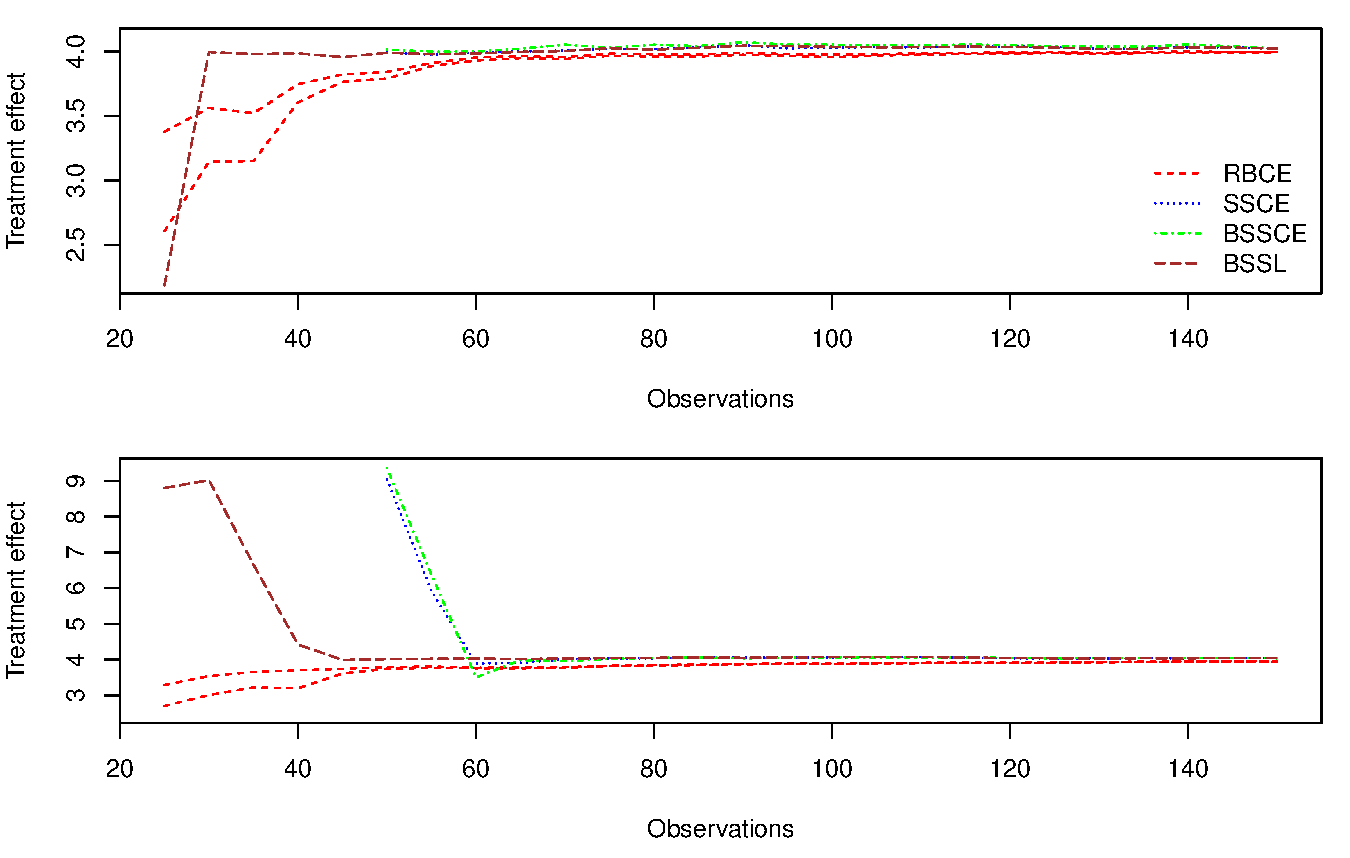
\includegraphics[width = 0.9\linewidth]{treat_obs.pdf}
    \caption{Comparison of different methods in estimating the causal effect for varying number of observations.}
    \label{fig:comp:trt}
\end{figure}

We also provide tables for the performance of variable selection in \cref{tab:misspec1,tab:misspec2}.
For variable selection, we use a loss function as described earlier.
Here, we consider
$\ell_1=\ell_2=1$ and $\ell_3= 0.2$,
i.e. we associate a loss of $1$ with false positive and false negative selections,
and a loss of $0.2$ with indeterminate selections.
Note that we could also choose more 
sophisticated loss functions based on \citep{ZAFFALON20121282}.
We sum these losses together across all predictors
to obtain the total loss, presented in \cref{tab:misspec1,tab:misspec2}.
The table counts the number of
false positives (FP) and false negatives (FN). For RBCE, we have an
additional column (ID)
which counts the number of indeterminate predictors.
From the table it can be seen that for the first scenario, our method
abstains from identifying some variables for 
$n \le 50$. Especially for $n=25$, our method identifies 39 and 35 variables as indeterminate
for the first setting and second setting respectively. However,
later on our method gives more precise results in terms of variable
selection. We also notice that the other methods tend to perform poorly
in terms of variable selection in the second case giving away many FNs. 
This can be seen in the bottom figure of \cref{fig:comp:trt}
as well.
% latex table generated in R 4.3.0 by xtable 1.8-4 package
% Wed May 24 00:50:53 2023
\begin{table}[ht]
\caption{Loss based on misspecification of active variables for first scenario.}\label{tab:misspec1}
\centering
\small
\begin{tabular}{|c||rrr|r||rr|r||rr|r||rr|r|}
  \hline
  &\multicolumn{4}{c||}{RBCE}&\multicolumn{3}{c||}{SSCE}
  &\multicolumn{3}{c||}{BSSCE}&\multicolumn{3}{c|}{BSSL}\\
  \cline{2-14}
 Obs & FP & FN & ID & Tot & FP & FN & Tot & FP & FN & Tot & FP & FN & Tot \\ 
  \hline
25 & 1 & 0 & 39 & 8.8 &  &  &  &  &  &  & 9 & 1 & 10 \\ 
  30 & 0 & 0 & 3 & 0.6 &  &  &  &  &  &  & 0 & 0 & 0 \\ 
  35 & 0 & 0 & 3 & 0.6 &  &  &  &  &  &  & 0 & 0 & 0 \\ 
  40 & 0 & 0 & 0 & 0 &  &  &  &  &  &  & 0 & 0 & 0 \\ 
  45 & 0 & 0 & 0 & 0 &  &  &  &  &  &  & 0 & 0 & 0 \\ 
  50 & 0 & 0 & 0 & 0 & 0 & 0 & 0 & 0 & 0 & 0 & 0 & 0 & 0 \\ 
  55 & 0 & 0 & 0 & 0 & 0 & 0 & 0 & 0 & 0 & 0 & 0 & 0 & 0 \\ 
  60 & 0 & 0 & 0 & 0 & 0 & 0 & 0 & 0 & 0 & 0 & 0 & 0 & 0 \\ 
  65 & 0 & 0 & 0 & 0 & 0 & 0 & 0 & 0 & 0 & 0 & 0 & 0 & 0 \\ 
  70 & 0 & 0 & 0 & 0 & 0 & 0 & 0 & 0 & 0 & 0 & 0 & 0 & 0 \\ 
  75 & 0 & 0 & 0 & 0 & 0 & 0 & 0 & 0 & 0 & 0 & 0 & 0 & 0 \\ 
  80 & 0 & 0 & 0 & 0 & 0 & 0 & 0 & 0 & 0 & 0 & 0 & 0 & 0 \\ 
  85 & 0 & 0 & 0 & 0 & 0 & 0 & 0 & 0 & 0 & 0 & 0 & 0 & 0 \\ 
  90 & 0 & 0 & 0 & 0 & 0 & 0 & 0 & 0 & 0 & 0 & 0 & 0 & 0 \\ 
  95 & 0 & 0 & 0 & 0 & 1 & 0 & 1 & 0 & 0 & 0 & 0 & 0 & 0 \\ 
  100 & 0 & 0 & 0 & 0 & 1 & 0 & 1 & 0 & 0 & 0 & 0 & 0 & 0 \\ 
  105 & 0 & 0 & 0 & 0 & 0 & 0 & 0 & 0 & 0 & 0 & 0 & 0 & 0 \\ 
  110 & 0 & 0 & 0 & 0 & 0 & 0 & 0 & 0 & 0 & 0 & 0 & 0 & 0 \\ 
  115 & 0 & 0 & 0 & 0 & 0 & 0 & 0 & 0 & 0 & 0 & 0 & 0 & 0 \\ 
  120 & 0 & 0 & 0 & 0 & 0 & 0 & 0 & 0 & 0 & 0 & 0 & 0 & 0 \\ 
  125 & 0 & 0 & 0 & 0 & 0 & 0 & 0 & 0 & 0 & 0 & 0 & 0 & 0 \\ 
  130 & 0 & 0 & 0 & 0 & 0 & 0 & 0 & 0 & 0 & 0 & 0 & 0 & 0 \\ 
  135 & 0 & 0 & 0 & 0 & 0 & 0 & 0 & 0 & 0 & 0 & 0 & 0 & 0 \\ 
  140 & 0 & 0 & 0 & 0 & 0 & 0 & 0 & 0 & 0 & 0 & 0 & 0 & 0 \\ 
  145 & 0 & 0 & 0 & 0 & 0 & 0 & 0 & 0 & 0 & 0 & 0 & 0 & 0 \\ 
  150 & 0 & 0 & 0 & 0 & 0 & 0 & 0 & 0 & 0 & 0 & 0 & 0 & 0 \\ 
   \hline
\end{tabular}
\end{table}
\begin{table}
\small
\caption{Loss based on misspecification of active variables for second scenario}
\label{tab:misspec2}
\begin{tabular}{|c||rrr|r||rr|r||rr|r||rr|r|}
  \hline
  &\multicolumn{4}{c||}{RBCE}&\multicolumn{3}{c||}{SSCE}
  &\multicolumn{3}{c||}{BSSCE}&\multicolumn{3}{c|}{BSSL}\\
  \cline{2-14}
 Obs & FP & FN & ID & Tot & FP & FN & Tot & FP & FN & Tot & FP & FN & Tot \\ 
  \hline
25 &   5 & 0 & 35 & 12 &  &  &  &  &  &  & 0 & 15 & 15 \\ 
  30 & 0 & 2 & 7 & 3.4 &  &  &  &  &  &  & 0 & 14 & 14 \\ 
  35 & 0 & 1 & 9 & 2.8 &  &  &  &  &  &  & 0 & 14 & 14 \\ 
  40 & 0 & 0 & 21 & 4.2 &  &  &  &  &  &  & 0 & 10 & 10 \\ 
  45 & 0 & 0 & 1 & 0.2 &  &  &  &  &  &  & 0 & 0 & 0 \\ 
  50 & 0 & 0 & 0 & 0 & 0 & 15 & 15 & 0 & 15 & 15 & 0 & 0 & 0 \\ 
  55 & 0 & 0 & 0 & 0 & 0 & 14 & 14 & 0 & 14 & 14 & 0 & 0 & 0 \\ 
  60 & 0 & 0 & 0 & 0 & 0 & 0 & 0 & 0 & 0 & 0 & 0 & 0 & 0 \\ 
  65 & 0 & 0 & 0 & 0 & 0 & 0 & 0 & 0 & 0 & 0 & 0 & 0 & 0 \\ 
  70 & 0 & 0 & 0 & 0 & 0 & 0 & 0 & 0 & 0 & 0 & 0 & 0 & 0 \\ 
  75 & 0 & 0 & 0 & 0 & 0 & 0 & 0 & 0 & 0 & 0 & 0 & 0 & 0 \\ 
  80 & 0 & 0 & 0 & 0 & 0 & 0 & 0 & 0 & 0 & 0 & 0 & 0 & 0 \\ 
  85 & 0 & 0 & 0 & 0 & 0 & 0 & 0 & 0 & 0 & 0 & 0 & 0 & 0 \\ 
  90 & 0 & 0 & 0 & 0 & 0 & 0 & 0 & 0 & 0 & 0 & 0 & 0 & 0 \\ 
  95 & 0 & 0 & 0 & 0 & 0 & 0 & 0 & 0 & 0 & 0 & 0 & 0 & 0 \\ 
  100 & 0 & 0 & 0 & 0 & 0 & 0 & 0 & 0 & 0 & 0 & 0 & 0 & 0 \\ 
  105 & 0 & 0 & 0 & 0 & 0 & 0 & 0 & 0 & 0 & 0 & 0 & 0 & 0 \\ 
  110 & 0 & 0 & 0 & 0 & 0 & 0 & 0 & 0 & 0 & 0 & 0 & 0 & 0 \\ 
  115 & 0 & 0 & 0 & 0 & 0 & 0 & 0 & 0 & 0 & 0 & 0 & 0 & 0 \\ 
  120 & 0 & 0 & 0 & 0 & 0 & 0 & 0 & 0 & 0 & 0 & 0 & 0 & 0 \\ 
  125 & 0 & 0 & 0 & 0 & 0 & 0 & 0 & 0 & 0 & 0 & 0 & 0 & 0 \\ 
  130 & 0 & 0 & 0 & 0 & 0 & 0 & 0 & 0 & 0 & 0 & 0 & 0 & 0 \\ 
  135 & 0 & 0 & 0 & 0 & 0 & 0 & 0 & 0 & 0 & 0 & 0 & 0 & 0 \\ 
  140 & 0 & 0 & 0 & 0 & 0 & 0 & 0 & 0 & 0 & 0 & 0 & 0 & 0 \\ 
  145 & 0 & 0 & 0 & 0 & 1 & 0 & 1 & 0 & 0 & 0 & 0 & 0 & 0 \\ 
  150 & 0 & 0 & 0 & 0 & 0 & 0 & 0 & 0 & 0 & 0 & 0 & 0 & 0 \\ 
  \hline
\end{tabular}
\end{table}

We show the result of our analyses with different number of predictors and
fixed number of sample in \cref{fig:comp:trt:pred,tab:causal2}. Similar to
the first two settings, we notice that our method is somewhat in agreement with
BSSL for the third setting. However, for the fourth setting, our method
underestimates the treatment effect significantly (5\% in the worst case). This
is somewhat in sync with the second setting, and a possible reason behind this
could be the fact that in both the cases, the number of active $\beta_j$'s is
higher than $\gamma_j$'s. This therefore, tends to reduce the value of treatment
effect. A possible way to work around this issue can be using the `DSS' estimates
of the regression coefficient and adjust the value of $\beta_T$. 

Besides this interesting result, we notice that all of the four methods perform
perfectly in variable selection giving no misspecified variables. Therefore,
we omit the table of variable selection for third and fourth scenarios.


% latex table generated in R 4.3.2 by xtable 1.8-4 package
% Mon Mar 25 10:08:22 2024
\begin{table}[ht]
\centering
\tiny
\caption{Comparison of different methods in estimating the causal effect for varying number of predictors.}
\begin{tabular}{c|ccccc|ccccc}
  \hline
 Case&  &  & 1 &  &  &  &  & 2 &  &  \\ 
  \hline
 & RBCE-l & RBCE-u & SSCE & BSSCE & BSSL & RBCE-l & RBCE-u & SSCE & BSSCE & BSSL \\ 
  \hline
\hline
30 & 3.93 & 3.95 & 3.99 & 4.00 & 3.99 & 3.89 & 3.90 & 4.02 & 4.02 & 4.01 \\ 
  35 & 3.93 & 3.94 & 3.99 & 3.99 & 3.99 & 3.88 & 3.91 & 4.02 & 4.01 & 4.02 \\ 
  40 & 3.93 & 3.95 & 3.99 & 4.01 & 3.99 & 3.89 & 3.91 & 4.01 & 4.03 & 4.01 \\ 
  45 & 3.93 & 3.95 & 3.99 & 4.01 & 3.99 & 3.89 & 3.91 & 4.02 & 4.02 & 4.02 \\ 
  50 & 3.94 & 3.95 & 3.99 & 4.00 & 3.99 & 3.89 & 3.91 & 4.01 & 4.02 & 4.02 \\ 
  55 & 3.94 & 3.95 & 3.99 & 4.00 & 3.98 & 3.89 & 3.91 & 4.02 & 4.02 & 4.02 \\ 
  60 & 3.94 & 3.95 & 3.99 & 4.01 & 3.99 & 3.89 & 3.91 & 4.02 & 4.02 & 4.02 \\ 
  65 & 3.94 & 3.94 & 3.99 & 4.00 & 3.98 & 3.89 & 3.91 & 4.02 & 4.03 & 4.02 \\ 
  70 & 3.93 & 3.95 & 3.99 & 4.00 & 3.99 & 3.89 & 3.90 & 4.02 & 4.02 & 4.02 \\ 
  75 & 3.92 & 3.94 & 3.99 & 4.00 & 3.99 & 3.89 & 3.90 & 4.01 & 4.02 & 4.02 \\ 
  80 & 3.92 & 3.94 & 3.99 & 3.99 & 3.99 & 3.89 & 3.90 & 4.01 & 4.01 & 4.02 \\ 
  85 & 3.92 & 3.94 & 3.99 & 4.00 & 3.98 & 3.88 & 3.90 & 4.02 & 4.02 & 4.02 \\ 
  90 & 3.92 & 3.93 & 3.99 & 4.00 & 3.99 & 3.88 & 3.90 & 4.02 & 4.01 & 4.02 \\ 
  95 & 3.92 & 3.94 & 3.99 & 4.00 & 3.98 & 3.87 & 3.90 & 4.02 & 4.01 & 4.02 \\ 
  100 & 3.92 & 3.94 & 3.99 & 3.99 & 3.98 & 3.88 & 3.90 & 4.02 & 4.02 & 4.01 \\ 
  105 & 3.92 & 3.94 &  &  & 3.98 & 3.86 & 3.90 &  &  & 4.02 \\ 
  110 & 3.92 & 3.94 &  &  & 3.99 & 3.87 & 3.90 &  &  & 4.01 \\ 
  115 & 3.91 & 3.94 &  &  & 3.98 & 3.87 & 3.90 &  &  & 4.02 \\ 
  120 & 3.91 & 3.94 &  &  & 3.99 & 3.87 & 3.91 &  &  & 4.02 \\ 
  125 & 3.91 & 3.94 &  &  & 3.99 & 3.87 & 3.89 &  &  & 4.02 \\ 
  130 & 3.92 & 3.94 &  &  & 3.99 & 3.86 & 3.90 &  &  & 4.01 \\ 
  135 & 3.90 & 3.93 &  &  & 3.98 & 3.86 & 3.90 &  &  & 4.01 \\ 
  140 & 3.91 & 3.93 &  &  & 3.99 & 3.85 & 3.89 &  &  & 4.01 \\ 
  145 & 3.90 & 3.94 &  &  & 3.98 & 3.84 & 3.89 &  &  & 4.01 \\ 
  150 & 3.90 & 3.93 &  &  & 3.99 & 3.85 & 3.88 &  &  & 4.02 \\ 
   \hline
\end{tabular}
\label{tab:causal2}
\end{table}

\begin{figure}
    \centering
    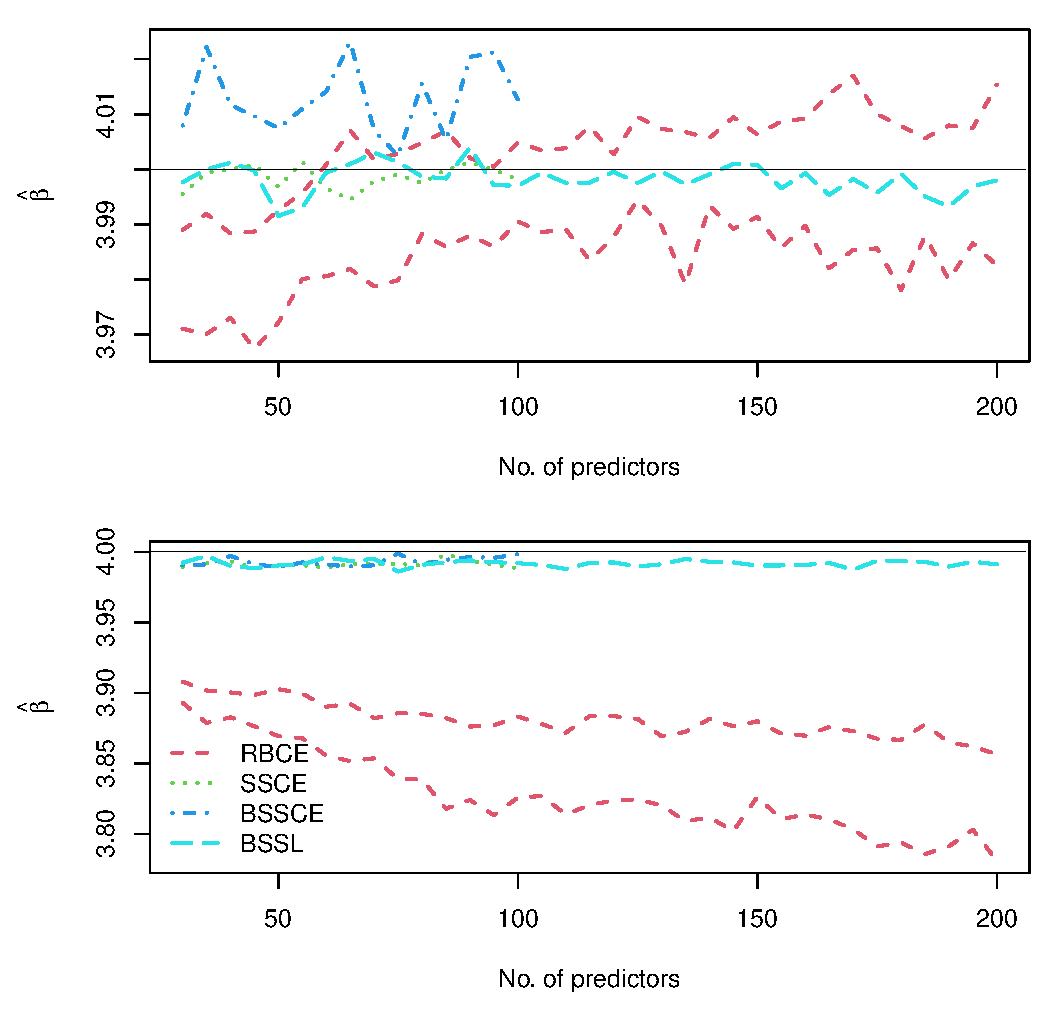
\includegraphics[width = 0.9\linewidth]{treat_pred.pdf}
    \caption{Comparison of different methods in estimating the causal effect for varying number of predictors.}
    \label{fig:comp:trt:pred}
\end{figure}



\section{Conclusion}\label{sec:conc}

Causal effect estimation is an important tool in statistical learning.
Especially in risk-sensitive situations, such as medicine, it needs to
be performed with utmost care as in many cases poor estimation can have severe adverse consequences.
In this paper, we tackle this issue by proposing a robust Bayesian analysis of the causal 
effect estimation problem for high dimensional data. Our 
framework is focused on the effect of prior elicitation on
%%% MT to TB: I don't understand "confounder selection" - do you mean
%%% "predictor selection" or "variable selection"? (also see later,
%%% "confounder selection" is repeated a few times; I'm not sure
%%% "confounder" is the correct term here, some variables may be
%%% confounding but some may not; if it is appropriate then earlier in
%%% the paper we should talk a bit more to explain why these variables
%%% are all confounders and be consistent with our terminology)
predictor selection
as well as causal effect estimation. We consider a spike and slab type
prior for predictor selection and discuss the possible sources of uncertainty that
need to be tackled carefully. We were particularly focused on the uncertainty associated
with prior selection probabilities for which we consider a set of beta priors to perform
sensitivity analysis. We showed that the sensitivity analysis on the prior selection probability
gives us a robust predictor selection scheme. In this way, we can abstain from selecting
a predictor when the available data is not sufficient. We also propose a generalised
utility based framework, where we associate a loss for abstaining which can be interpreted 
as the cost of further data collection. Finally, we illustrate our method with synthetic dataset
and compare with other state of the art Bayesian methods. 


Currently, the paper proposes a robust Bayesian approach for causal effect estimation where
we rely on sampling strategies to obtain the posterior bounds as well as performing 
variable selection. In future, it will be interesting to derive inner approximation bounds
for the posterior estimates to reduce the computational cost,
or to find better ways than brute force optimisation, such as for instance iterative importance sampling \citep{cruz22_importance}. Moreover, for the sake of
illustration, we rely on simple loss functions
%TB to MT: edited the conclusion
associated with the predictor selection. However,
this paradigm can be used for a generalised
decision theoretic framework as well where based on
the predictor selection we can formulate the 
problem as a decision support problem for treating a subject.

We also notice with our simulation studies that our
method tends to underestimate the causal effect
when some predictors are only associated with the
outcome model. This suggests that we might want
to use a correction formula for the causal effect.
Moreover, in future, we would
like to investigate different elicitation strategies for different prior parameters and their importance in causal effect estimation. 


In general, we noticed that our method
is in good agreement with other methods with an added level of robustness.
This shows that our method has good potential for real-life problems,
and we intend to apply it on a real dataset in future work.

\section*{Acknowledgements}

We sincerely thank Jochen Einbeck for his contributions to an earlier version of this paper.

\bibliographystyle{elsarticle-num-names} 
\bibliography{basu_causal}

\end{document}
